
\documentclass{beamer}

\usepackage{graphicx}
\usepackage{tikz}
\usetikzlibrary{arrows}

\newtheorem{thm}{Theorem}
\newtheorem{prop}[thm]{Proposition}

\newenvironment{defn}[1][Definition]{\begin{trivlist}
\item[\hskip \labelsep {\bfseries #1}]}{\end{trivlist}}

\newcommand{\R}{\mathbb{R}}
\newcommand{\T}{\mathcal{T}}
\newcommand{\B}{\mathbb{B}}
\newcommand{\n}{$n$}
\newcommand{\Y}{\Gamma_Y}
\newcommand{\C}{$C^2(\Y)$}


\usetheme{Madrid}


\title{Collision Avoidance on Finite Graphs}

\subtitle{Retracting Space to Save Robots}

\author{Tynan Daly}


\institute[Bates College] 

\date{December 2, 2014}


\subject{Applied Computational Topology}
% This is only inserted into the PDF information catalog. Can be left
% out. 

% If you have a file called "university-logo-filename.xxx", where xxx
% is a graphic format that can be processed by latex or pdflatex,
% resp., then you can add a logo as follows:

% \pgfdeclareimage[height=0.5cm]{university-logo}{university-logo-filename}
% \logo{\pgfuseimage{university-logo}}

% Delete this, if you do not want the table of contents to pop up at
% the beginning of each subsection:
\AtBeginSubsection[]
{
  \begin{frame}<beamer>{Outline}
    \tableofcontents[currentsection,currentsubsection]
  \end{frame}
}

% Let's get started
\begin{document}

\begin{frame}
  \titlepage
\end{frame}

\begin{frame}{Outline}
  \tableofcontents
  % You might wish to add the option [pausesections]
\end{frame}

% Section and subsections will appear in the presentation overview
% and table of contents.

\section{The Problem at Hand}
\begin{frame}{Our Problem}
\begin{itemize}
\item In order to carry out tasks, robots needs to go from point $a$ to point $b$ without colliding.\pause
\item The more robots in a given space, the more complex their possible configurations become.\pause
\item As a result, algorithmic tools used to find safe configurations become increasingly inefficient.\pause
\item We need tractable problems. We must simplify our possible configurations. 
\end{itemize}
\end{frame}

\begin{frame}{Different Types of Robotic Movement}
  \begin{itemize}
  \item Unrestricted --- Self driving cars\pause
  
  \item Restricted --- Robots in a factory
  \end{itemize}
\end{frame}

\section{Configuration Spaces}

\begin{frame}{Configuration Space}
\begin{itemize}
\item We call the collection of all possible configurations the \textbf{configuration space}.
\item Given a space $X$, we define the configuration space of $N$ robots to be \pause
\begin{align*}
C^N(X)=(\underbrace{X_1\times X_2 \times\dots \times X_N}_{N \text{ times}}) - \Delta
\end{align*}
\pause 
where 
\begin{align*}
\Delta = \{ (x_1,x_2,\dots,x_N)| x_i=x_j \text{ for some } i\neq j\}.
\end{align*}
\end{itemize}
\end{frame}

\begin{frame}{Why use the Configuration Space?}
\begin{itemize}
\item Configuration spaces make the complex simple.\pause
\item We can apply mathematical tools to them.
\end{itemize}
\end{frame}


\begin{frame}{Simple Robots}

\begin{itemize}
\item Let us consider two simple robots which can only move backwards and forwards in a straight line.\pause
\item What does their configuration space look like? \pause

\centering
\includegraphics[scale=.25]{xygraph.jpg}
\begin{align*}
C^2(\mathbb{R})=\mathbb{R}^2 - \{(x_1,x_2)|x_1=x_2\}
\end{align*}
\end{itemize}

\end{frame}

\begin{frame}{More Complicated Robots}
\begin{itemize}
\item What about three robots that can move around in two dimensions, such as self driving cars?\pause
\item This configuration space, $C^3(\R^2)$, exists in six dimensions.
\end{itemize}

 
\end{frame}


\subsection{Fixed Movement Networks}

\begin{frame}{Robots with Fixed Movement Paths}
\begin{itemize}
\item Can most robots move around freely?\pause
\item Most robots move along fixed movement networks.
\end{itemize}
\end{frame}

\begin{frame}{Robots with Fixed Movement Paths}
\begin{itemize}
\item Let us consider the movement network $\Y$.
\end{itemize}
\begin{figure}[h]
\caption{The graph $\Y$}
\centering
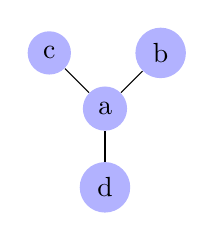
\begin{tikzpicture}
  [scale=.7,auto=left,every node/.style={circle,fill=blue!30}]
  \node (n1) {a};
  \node (n2) [above right of=n1]  {b};
  \node (n3) [above left of=n1] {c};
  \node (n4) [below of=n1] {d};

\foreach \from/\to in
{n1/n3,n2/n1,n4/n1}
    \draw (\from) -> (\to);
\end{tikzpicture}
\label{fig:maze}
\end{figure}
\end{frame}

\begin{frame}{Why $\Y$?}
\begin{itemize}
\item One of the simplest non-trivial examples.
\item Many movement networks can be built from joining multiple ``Y'' graphs together. 
\end{itemize}
\end{frame}

\begin{frame}{Visualizing $C^2(\Y)$}
\begin{itemize}
\item What does $C^2(\Y)$ look like? \pause


\centering
\includegraphics[scale=.75]{Config.jpg}
\end{itemize}
\end{frame}

\begin{frame}{Keep It Simple Students}
\begin{itemize}
\item We cannot use graph theory tools on this space.\pause
\item But by \textbf{discretizing} \C, we can obtain something much more tractable.
\end{itemize}
\end{frame}

\begin{frame}{The Discretized Configuration Space}
\begin{itemize}
\item The discretized configuration space, $\mathcal{D}^N(X)$ is defined as 
\begin{align*}
\mathcal{D}^N(X) = (\underbrace{X\times X \times \dots \times X}_{N\text{ times}}) - \tilde{\Delta} 
\end{align*}\pause
where $\tilde{\Delta}$ is the collection of all cells whose closure intersects the pairwise diagonal.
\end{itemize}
\end{frame}

\begin{frame}{Visualizing $\mathcal{D}^2(\Y)$}
\centering
\includegraphics[scale=.75]{discretized.jpg}
\end{frame}

\begin{frame}{We Can Do Better}
\begin{itemize}
\item Not all configuration spaces are as easy to visualize as \C.\pause
\item We need to generalize our method of discretization. 
\end{itemize}
\end{frame}

\section{Building \C}
\subsection{CW Complexes}
\begin{frame}{CW Complexes}
\begin{itemize}
\item To build $C^2(\Y)$ we need to first discuss CW complexes.\pause
\end{itemize}

\begin{block}{Definition.}
A CW complex is any space $X$ which can be built by starting off with a discrete collection of points called $X^0$, then attaching one-dimensional disks $D^1$ to $X^0$ along their boundaries $S^0$, writing $X^1$ for the object obtained by attaching the $D^1$s to $X^0$, then attaching two-dimensional disks $D^2$ to $X^1$ along their boundaries $S^1$, writing $X^2$ for the new space, and so on, giving spaces $X^N$ for every $N$~\cite{CW}.
\end{block}
\end{frame}

\begin{frame}{What does that mean?}
\begin{itemize}
\item To form a CW complex of dimension $N$, we begin with a collection of $0$-cells called $X^0$.\pause
\item We use $X^0$ to form $X^1$, $X^1$ to form $X^2$, and so on... \pause
\item Since we are dealing with real world applications, this process repeats a finite number of times until we arrive at $X^N$. \pause
\item To illustrate, we will begin to build \C.
\end{itemize}
\end{frame}

\subsection{Building $\Y \times \Y$.}
\begin{frame}{Names and Labels}
\begin{itemize}
\item Consider the sub-graph of $\Y$ where robot $1$ only moves between nodes $a$ and $b$ and robot $2$ only moves between $a$ and $c$.
\pause
\begin{figure}[h]
\caption{Sub-graphs of $\Y$.}\label{fig:1cells}
\centering

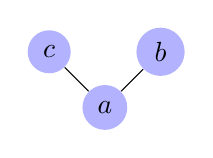
\begin{tikzpicture}
  [scale=.7,auto=left,every node/.style={circle,fill=blue!30}]
  \node (n1) {$a$};
  \node (n2) [above right of=n1]  {$b$};
  \node (n3) [above left of=n1] {$c$};

\foreach \from/\to in
{n1/n2, n1/n3}
    \draw (\from) -> (\to);
\end{tikzpicture}\pause \hspace{2cm}
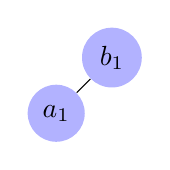
\begin{tikzpicture}
  [scale=.7,auto=left,every node/.style={circle,fill=blue!30}]
  \node (n1) {$a_1$};
  \node (n2) [above right of=n1]  {$b_1$};

\foreach \from/\to in
{n1/n2}
    \draw (\from) -> (\to);
\end{tikzpicture}
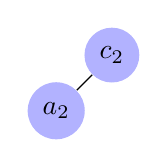
\begin{tikzpicture}
  [scale=.7,auto=left,every node/.style={circle,fill=blue!30}]
  \node (n1) {$a_2$};
  \node (n2) [above right of=n1]  {$c_2$};

\foreach \from/\to in
{n1/n2}
    \draw (\from) -> (\to);
\end{tikzpicture}
\end{figure}

\end{itemize}
\end{frame}

\begin{frame}{Cross Product of Vertices}
We form our collection of $0$-cells by taking cross products of their vertices.
\begin{figure}
\centering
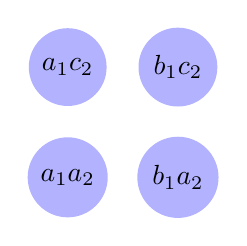
\begin{tikzpicture}
  [scale=.7,auto=left,every node/.style={circle,fill=blue!30}]
  \node (n1) at (1,3)  {$a_1c_2$};
  \node (n2) at (3,3)  {$b_1c_2$};
  \node (n3) at (1,1)  {$a_1a_2$};
  \node (n4) at (3,1)  {$b_1a_2$};


\end{tikzpicture}
\end{figure}

\end{frame}

\begin{frame}{Cross Product of Vertices and Edges}
We then add interior of the edges, our $1$-cells, to their boundaries.

\begin{figure}
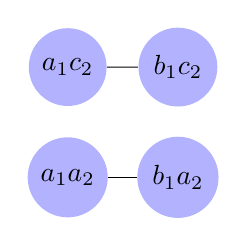
\begin{tikzpicture}
  [scale=.7,auto=left,every node/.style={circle,fill=blue!30}]
  \node (n1) at (1,3)  {$a_1c_2$};
  \node (n2) at (3,3)  {$b_1c_2$};
  \node (n3) at (1,1)  {$a_1a_2$};
  \node (n4) at (3,1)  {$b_1a_2$};
\foreach \from/\to in
{n1/n2, n3/n4}
    \draw (\from) -> (\to);


\end{tikzpicture}\pause
\hspace{.5in}
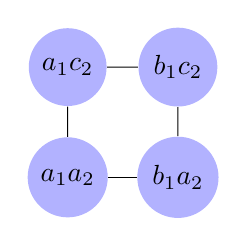
\begin{tikzpicture}
  [scale=.7,auto=left,every node/.style={circle,fill=blue!30}]
  \node (n1) at (1,3)  {$a_1c_2$};
  \node (n2) at (3,3)  {$b_1c_2$};
  \node (n3) at (1,1)  {$a_1a_2$};
  \node (n4) at (3,1)  {$b_1a_2$};

\foreach \from/\to in
{n1/n2, n3/n4, n1/n3, n2/n4}
    \draw (\from) -> (\to);

\end{tikzpicture}
\end{figure}
\end{frame}

\begin{frame}{A $2$-Cell}
Next we attach the cross product of the edges, the $2$-cell, to its boundary. 

\begin{figure}
\centering
 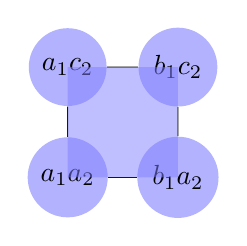
\begin{tikzpicture}
  [scale=.7,auto=left,every node/.style={circle,fill=blue!30}]
  \node (n1) at (1,3)  {$a_1c_2$};
  \node (n2) at (3,3)  {$b_1c_2$};
  \node (n3) at (1,1)  {$a_1a_2$};
  \node (n4) at (3,1)  {$b_1a_2$};

\foreach \from/\to in
{n1/n2, n3/n4, n1/n3, n2/n4}
    \draw (\from) -> (\to);
    \path[fill=blue!50,opacity=.5] (n1.center) to (n2.center) to (n4.center) to (n3.center) to (n1.center);
\end{tikzpicture}
\end{figure}
\end{frame}

\begin{frame}{Repeat}
\begin{itemize}
\item We can do this for another subgraph of $\Y$.\pause

\centering
 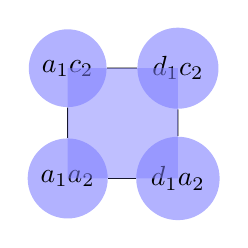
\begin{tikzpicture}
  [scale=.7,auto=left,every node/.style={circle,fill=blue!30}]
  \node (n1) at (1,3)  {$a_1c_2$};
  \node (n2) at (3,3)  {$d_1c_2$};
  \node (n3) at (1,1)  {$a_1a_2$};
  \node (n4) at (3,1)  {$d_1a_2$};

\foreach \from/\to in
{n1/n2, n3/n4, n1/n3, n2/n4}
    \draw (\from) -> (\to);
    \path[fill=blue!50,opacity=.5] (n1.center) to (n2.center) to (n4.center) to (n3.center) to (n1.center);
\end{tikzpicture}
\end{itemize}
\end{frame}

\begin{frame}{Attaching $2$-cells}
\begin{itemize}
\item We then attach our $2$-cells along their common vertices and edges. \pause 

\centering
 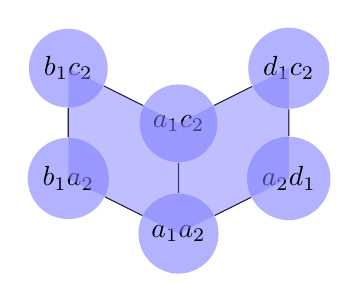
\begin{tikzpicture}
  [scale=.7,auto=left,every node/.style={circle,fill=blue!30}]
  \node (n1) at (1,2)  {$b_1a_2$};
  \node (n2) at (1,4)  {$b_1c_2$};
  \node (n3) at (3,1)  {$a_1a_2$};
  \node (n4) at (3,3)  {$a_1c_2$};
  \node (n5) at (5,4)  {$d_1c_2$};
  \node (n6) at (5,2)  {$a_2d_1$};


\foreach \from/\to in
{n1/n3, n2/n4, n1/n2, n4/n3, n4/n5, n5/n6, n6/n3}
    \draw (\from) -> (\to);
    \path[fill=blue!50,opacity=.5] (n1.center) to (n2.center) to (n4.center) to (n3.center) to (n1.center);
    \path[fill=blue!50,opacity=.5] (n4.center) to (n5.center) to (n6.center) to (n3.center) to (n4.center);
\end{tikzpicture}
\end{itemize}
\end{frame}

\begin{frame}{And Repeat Again...}
\begin{itemize}
\item We can do this process again.\pause 

\centering
 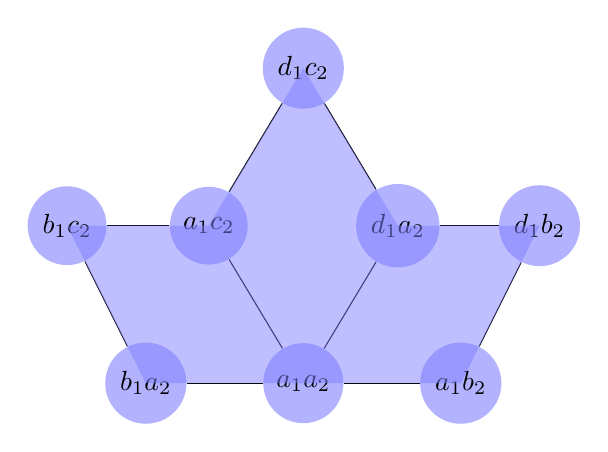
\begin{tikzpicture}
  [scale=1,auto=left,every node/.style={circle,fill=blue!30}]
  \node (n1) at (1,0)    {$b_1a_2$};
  \node (n2) at (0,2)    {$b_1c_2$};
  \node (n3) at (3,0)    {$a_1a_2$};
  \node (n4) at (1.8,2)  {$a_1c_2$};
  \node (n5) at (3,4)    {$d_1c_2$};
  \node (n6) at (4.2,2)  {$d_1a_2$};
  \node (n7) at (6,2)    {$d_1b_2$};
  \node (n8) at (5,0)    {$a_1b_2$};

\foreach \from/\to in
{n1/n3, n2/n4, n1/n2, n4/n3, n4/n5, n5/n6, n6/n3, n6/n7, n7/n8, n8/n3}
    \draw (\from) -> (\to);
    \path[fill=blue!50,opacity=.5] (n1.center) to (n2.center) to (n4.center) to (n3.center) to (n1.center);
    \path[fill=blue!50,opacity=.5] (n4.center) to (n5.center) to (n6.center) to (n3.center) to (n4.center);
    \path[fill=blue!50,opacity=.5] (n3.center) to (n6.center) to (n7.center) to (n8.center) to (n3.center);
\end{tikzpicture}
\end{itemize}
\end{frame}

\begin{frame}{Six Attached $2$-cells}

\centering
 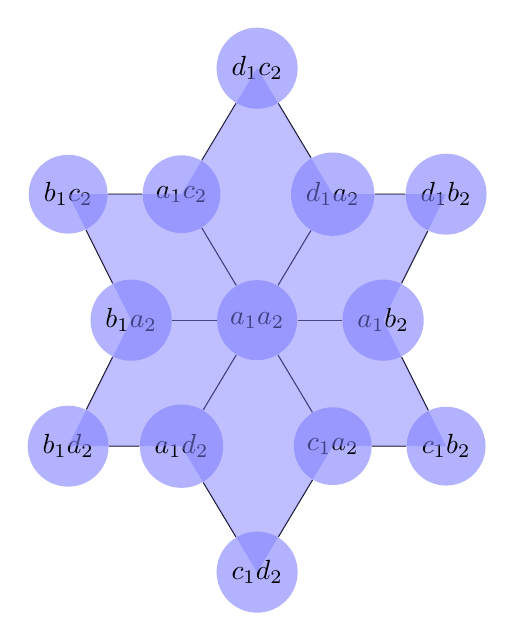
\begin{tikzpicture}
  [scale=.8,auto=left,every node/.style={circle,fill=blue!30}]
  \node (n1) at (1,0)       {$b_1a_2$};
  \node (n2) at (0,2)       {$b_1c_2$};
  \node (n3) at (3,0)       {$a_1a_2$};
  \node (n4) at (1.8,2)     {$a_1c_2$};
  \node (n5) at (3,4)       {$d_1c_2$};
  \node (n6) at (4.2,2)     {$d_1a_2$};
  \node (n7) at (6,2)       {$d_1b_2$};
  \node (n8) at (5,0)       {$a_1b_2$};
  
  \node (n9) at (0,-2)      {$b_1d_2$};
  \node (n10) at (1.8, -2)  {$a_1d_2$};
  \node (n11) at (3,-4)     {$c_1d_2$};
  \node (n12) at (4.2, -2)  {$c_1a_2$};
  \node (n13) at (6,-2)     {$c_1b_2$};

\foreach \from/\to in
{n1/n3, n2/n4, n1/n2, n4/n3, n4/n5, n5/n6, n6/n3, n6/n7, n7/n8, n8/n3, n1/n9, n9/n10, n10/n3, n10/n11, n11/n12, n12/n3, n12/n13, n13/n8}
    \draw (\from) -> (\to);
    \path[fill=blue!50,opacity=.5] (n1.center) to (n2.center) to (n4.center) to (n3.center) to (n1.center);
    \path[fill=blue!50,opacity=.5] (n4.center) to (n5.center) to (n6.center) to (n3.center) to (n4.center);
    \path[fill=blue!50,opacity=.5] (n3.center) to (n6.center) to (n7.center) to (n8.center) to (n3.center);
    \path[fill=blue!50,opacity=.5] (n1.center) to (n9.center) to (n10.center) to (n3.center) to (n1.center);
    \path[fill=blue!50,opacity=.5] (n3.center) to (n10.center) to (n11.center) to (n12.center) to (n3.center);
    \path[fill=blue!50,opacity=.5] (n3.center) to (n12.center) to (n13.center) to (n8.center) to (n3.center);
\end{tikzpicture}
\end{frame}

\begin{frame}{$\Y \times \Y$}
\centering
 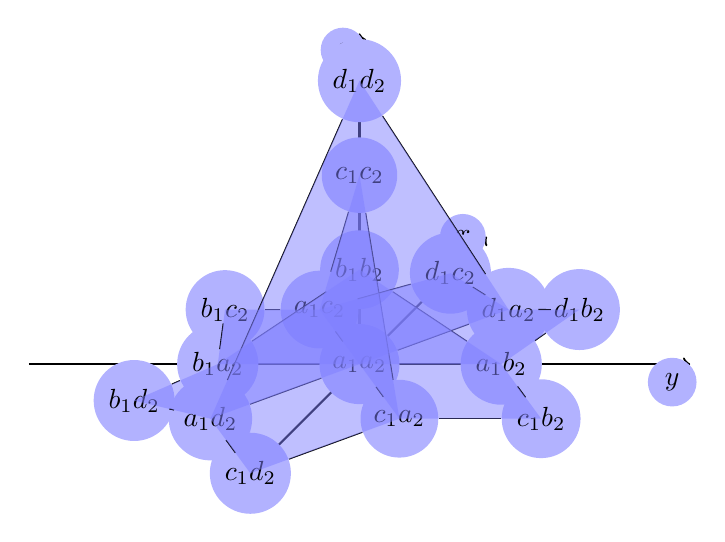
\begin{tikzpicture}
  [scale=.60,auto=left,every node/.style={circle,fill=blue!30}]
  \draw[thick,->,black] (-7,0,0) -- (7,0,0) node[anchor=north east]{$y$};
  \draw[thick,->] (0,0,0) -- (0,7,0) node[anchor=north east]{$z$};
  \draw[thick,->] (0,0,7) -- (0,0,-7) node[anchor=east]{$x$};
  
  \node (n0) at (0,0,0)         {$a_1a_2$};
  \node (n1) at (0,0,-5)        {$d_1c_2$};
  \node (n2) at (0,0,6)         {$c_1d_2$};
  \node (n3) at (-3,0,0)        {$b_1a_2$};
  \node (n4) at (3,0,0)         {$a_1b_2$};
  \node (n5) at (-4,0, 2)       {$b_1d_2$};
  \node (n6) at (-2,0, 3)       {$a_1d_2$};
  \node (n7) at (-4,0,-3)       {$b_1c_2$};
  \node (n8) at (-2,0,-3)       {$a_1c_2$};
  \node (n9) at (2,0, 3)        {$c_1a_2$};
  \node (n10) at (5, 0, 3)      {$c_1b_2$};
  \node (n11) at (3.5, 0, -3)   {$d_1b_2$};
  \node (n12) at (2, 0, -3)     {$d_1a_2$};
  \node (n13) at (0, 6, 0)      {$d_1d_2$};
  \node (n14) at (0, 4, 0)      {$c_1c_2$};
  \node (n15) at (0,2,0)        {$b_1b_2$};
  
  \foreach \from/\to in
{n0/n8, n0/n9, n0/n6, n0/n12, n0/n3, n0/n4, n4/n11, n11/n12, n4/n10, n10/n9, n12/n1, n1/n8, n8/n7, n7/n3, n3/n5, n5/n6, n6/n2, n2/n9, n6/n13, n13/n12, n8/n14, n14/n9, n3/n15, n15/n4}
    \draw (\from) -> (\to);
    \path[fill=blue!50,opacity=.5] (n1.center) to (n12.center) to (n11.center) to (n4.center) to (n10.center) to (n9.center) to (n2.center) to (n6.center) to (n5.center) to (n3.center) to (n7.center) to (n8.center) to (n1.center);
    \path[fill=blue!50,opacity=.5] (n6.center) to (n13.center) to (n12.center) to (n6.center);
    \path[fill=blue!50,opacity=.5] (n8.center) to (n14.center) to (n9.center) to (n8.center);
    \path[fill=blue!50,opacity=.5] (n3.center) to (n15.center) to (n4.center) to (n3.center);
\end{tikzpicture}
\end{frame}

\subsection{Removing the Pairwise Diagonal}

\begin{frame}{Removing $\Delta$}
\begin{itemize}
\item In order to turn the product space of $\Y \times \Y$ into \C, we must remove $\Delta$. \pause
\item Recall that 
\begin{align*}
\Delta = \{ (x_1,x_2,\dots,x_n)| x_i=x_j \text{ for some } i\neq j\}.
\end{align*}\pause
\centering
 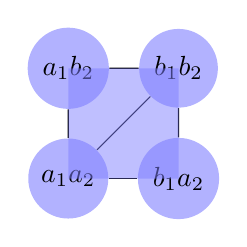
\begin{tikzpicture}
  [scale=.7,auto=left,every node/.style={circle,fill=blue!30}]
  \node (n1) at (1,3)  {$a_1b_2$};
  \node (n2) at (3,3)  {$b_1b_2$};
  \node (n3) at (1,1)  {$a_1a_2$};
  \node (n4) at (3,1)  {$b_1a_2$};

\foreach \from/\to in
{n1/n2, n3/n4, n1/n3, n2/n4, n2/n3}
    \draw (\from) -> (\to);
    \path[fill=blue!50,opacity=.5] (n1.center) to (n2.center) to (n4.center) to (n3.center) to (n1.center);
\end{tikzpicture}
\end{itemize}
\end{frame}

\begin{frame}{And Repeat}
\begin{itemize}
\item Doing this to every $2$-cell yields \C.
\end{itemize}

\centering
\includegraphics[scale=.75]{Config.jpg}
\end{frame}

\section{Obtaining $\mathcal{D}^2(\Y)$}
\subsection{Generalized Discretization}

\begin{frame}{Deformation Retract}
\begin{block}{Definition}
Let $X$ be a topological space with $A\subseteq X$, let $i\colon A\hookrightarrow X$ be the inclusion function, the function given by $i(a)=a$ for every $a$ in $A$, and let $f\colon X\rightarrow A$ be a continuous function such that $f(a)= a$ for all $a\in A$. We say $A$ is a deformation retract of $X$ and that function $i\circ f\colon X\rightarrow X$ is a deformation retraction if $i\circ f \simeq Id_X$ such that the homotopy function fixes every point in $A$.
\end{block}
\end{frame}

\begin{frame}{Deformation Retract Explained}
\begin{itemize}
\item The homotopy is a function $F:X \times I \to X$ which satisfies the four conditions:
\begin{enumerate}
\item $F(x,0)=Id_X(x)=x$ for all $x \in X$;

\item $F(x,1)=f(x)=i(f(x))$ for all $x\in X$;

\item $F$ is continuous;
\item $F(a,t)=a$ for all $t$.
\end{enumerate}\pause

\item Just like the movies.
\end{itemize}
\end{frame}

\subsection{Retracting \C}

\begin{frame}{Retracting \C}
\begin{itemize}
\item We begin with \C.\pause
\end{itemize}
\centering
\includegraphics[scale=.75]{Config.jpg}
\end{frame}

\begin{frame}{The First Retraction}
\begin{itemize}
\item We first retract every $2$-cell onto it's boundary.\pause
\end{itemize}

\centering
\includegraphics[scale=1]{Thesis/Twins.png}
\end{frame}

\begin{frame}{The First Retraction}
\centering
\includegraphics[scale=.6]{Thesis/NoInt.png}
\end{frame}

\begin{frame}{The Second Retraction}
\begin{itemize}
\item We then retract every open $1$-cell onto its boundary.\pause
\end{itemize}

\centering
\includegraphics[scale=.5]{Thesis/discretized.png}
\end{frame}

\section{Successful Simplification}
\subsection{Poorly Behaved Spaces}

\begin{frame}{The Good, the Bad, and the Disconnected}

\begin{itemize}
\item Not all spaces retract into such nice discretized configuration spaces.\pause
\end{itemize}

\begin{figure}
\centering
\includegraphics{Thesis/Bad.png}
\caption{The Graph $\Psi$}
\end{figure}
\end{frame}

\begin{frame}{$C^2(\Psi)$}
\begin{itemize}
\item We use a similar procedure to construct $C^2(\Psi)$.\pause
\end{itemize}

\centering
\includegraphics[scale=.5]{Thesis/Bad_C.png}

\end{frame}


\begin{frame}{$\mathcal{D}^2(\Psi)$}
\begin{itemize}
\item Discretizing $C^2(\Psi)$ yields two disconnected graphs.\pause
\end{itemize}

\centering
\includegraphics[scale=.5]{Thesis/Bad_D.png}

\end{frame}

\subsection{When Retraction Works}
\begin{frame}{A Sure Thing}
\begin{thm}
For any $N$ robots with $N>1$, on a graph $\Gamma$ with at least $N$ vertices, $C^N(\Gamma)$ retracts onto $D^N(\Gamma)$ if and only if 

\begin{enumerate}
\item Each path between distinct essential vertices passes through at least $N-1$ edges; and,
\item Each cycle not homotopic to a point passes through at least $N+1$ edges.\cite{factory}
\end{enumerate}
\end{thm}

\vspace{.5cm}
\centering
\includegraphics[scale=.8]{Thesis/Bad.png}
\end{frame}

\begin{frame}{Bounding the Dimension of $\mathcal{D}^N{X}$}
\begin{thm} \label{thm:dim}
Given a graph $G$ with $V$ vertices of degree two or greater, the discretization of $C^N(G)$ has a dimension of at most $V$.~\cite{factory}
\end{thm}
\end{frame}

\section{Concluding Remarks}
\begin{frame}{Concluding Remarks}
\begin{enumerate}
\item The takeaway.\pause
\item Further work.
\end{enumerate}
\end{frame}


% All of the following is optional and typically not needed. 
\appendix
\section<presentation>*{\appendixname}
\subsection<presentation>*{For Further Reading}

\begin{frame}[allowframebreaks]
  \frametitle<presentation>{For Further Reading}
    
  \begin{thebibliography}{10}
    
  \beamertemplatebookbibitems
  % Start with overview books.
  
    
  \bibitem{ed}
    H.~Edelsbrunner and J.~Harer.
    \newblock {\em Computational Topology: An Introduction}.
    \newblock American Mathematical Society, 2009.
    
  
    
    \bibitem{top}
        C. Adams and R. Franzosa
        \newblock Introduction to Topology: Pure and Applied
        \newblock Pearson, Inc.
    
    \bibitem{cw}
        R. Fritsch and R. Piccinini
        \newblock Cellular Structures in Topology
        \newblock Cambridge University Press
    
    \bibitem{at}
        A. Hatcher
        \newblock Algebraic Topology
        \newblock Cambridge University Press
    
  \beamertemplatearticlebibitems
  
  \bibitem{CW}
    E.~Weisstein.
    \newblock CW-Complex
    \newblock {\em  MathWorld--A Wolfram Web Resource}, Ret.           11/27/2014.
    \newblock http://mathworld.wolfram.com/CW-Complex.html
    
    \bibitem{factory}
        A. Abrams and R. Ghrist
        \newblock Finding Topology in a Factory: Configuration             Spaces
        \newblock The American Mathematical Monthly
    
    \bibitem{thesis}
        A. Abrams
        \newblock Configuration Spaces and Braid Groups of Graphs
        \newblock University Of California at Berkley
  % Followed by interesting articles. Keep the list short. 



  \end{thebibliography}
\end{frame}

\end{document}
